%------------------ vorlage.tex ------------------------------------------------
%
% LaTeX-Vorlage zur Erstellung von Projektdokumentationen
% im Fachbereich Informatik der Hochschule Trier
%
% Basis: Vorlage 'svmono' des Springer Verlags
% Bearbeiter: Hermann Schloß, Christian Bettinger
%
%-------------------------------------------------------------------------------


%------------------ Präambel ---------------------------------------------------
\documentclass[envcountsame,envcountchap deutsch]{i-studis}

\usepackage[utf8]{inputenc}

\usepackage[a4paper]{geometry}
\usepackage[english, ngerman]{babel}

\usepackage[pdftex]{graphicx}
\usepackage{epstopdf}

\usepackage{listings}

\usepackage[german, ruled, vlined]{algorithm2e}
\usepackage{amssymb, amsfonts, amstext, amsmath}
\usepackage{array}
\usepackage[skip=10pt]{caption}
\usepackage[usenames, dvipsnames]{color}
\usepackage[pdftex, plainpages=false]{hyperref}
\usepackage{textcomp}
\usepackage{hyperref}
\usepackage{graphicx}
\usepackage{fancyhdr}
\usepackage{algorithmic}

\usepackage{bibgerm}
\bibliographystyle{geralpha}

\usepackage{makeidx}
\usepackage{multicol}
\makeindex

\pagestyle{myheadings}
\setlength{\textheight}{1.1\textheight}
\setlength{\parindent}{0pt}

\lstset{
	language=[Sharp]C,
	basicstyle=\scriptsize\ttfamily,
	commentstyle=\scriptsize\ttfamily\color{Gray},
	identifierstyle=\scriptsize\ttfamily,
	keywordstyle=\scriptsize\ttfamily,
	stringstyle=\scriptsize\ttfamily,
	tabsize=4,
	numbers=left,
	numberstyle=\tiny,
	numberblanklines=false,
	frame=single,
	framesep=3mm,
	framexleftmargin=7mm,
	xleftmargin=10mm,
	linewidth=144mm,
	captionpos=b,
}



%------------------ Manuelle Silbentrennung ------------------------------------
%\hyphenation{Ele-men-tar-ob-jek-te ab-ge-tas-tet Aus-wer-tung House-holder-Matrix Least-Squares-Al-go-ri-th-men}
\definecolor{meinefarbe}{RGB}{249, 248, 113}
\color{meinefarbe}


\definecolor{hintergrund}{RGB}{0, 13, 0}
\pagecolor{hintergrund}
%------------------ Titelseite -------------------------------------------------
\begin{document}
\begin{titlepage}
 
\begin{center}
	{\Huge\bfseries Game Design Dokument} \\
	{\Huge\bfseries für Thorned King} \\
	
\end{center}

\begin{figure}[h]
	\centering
	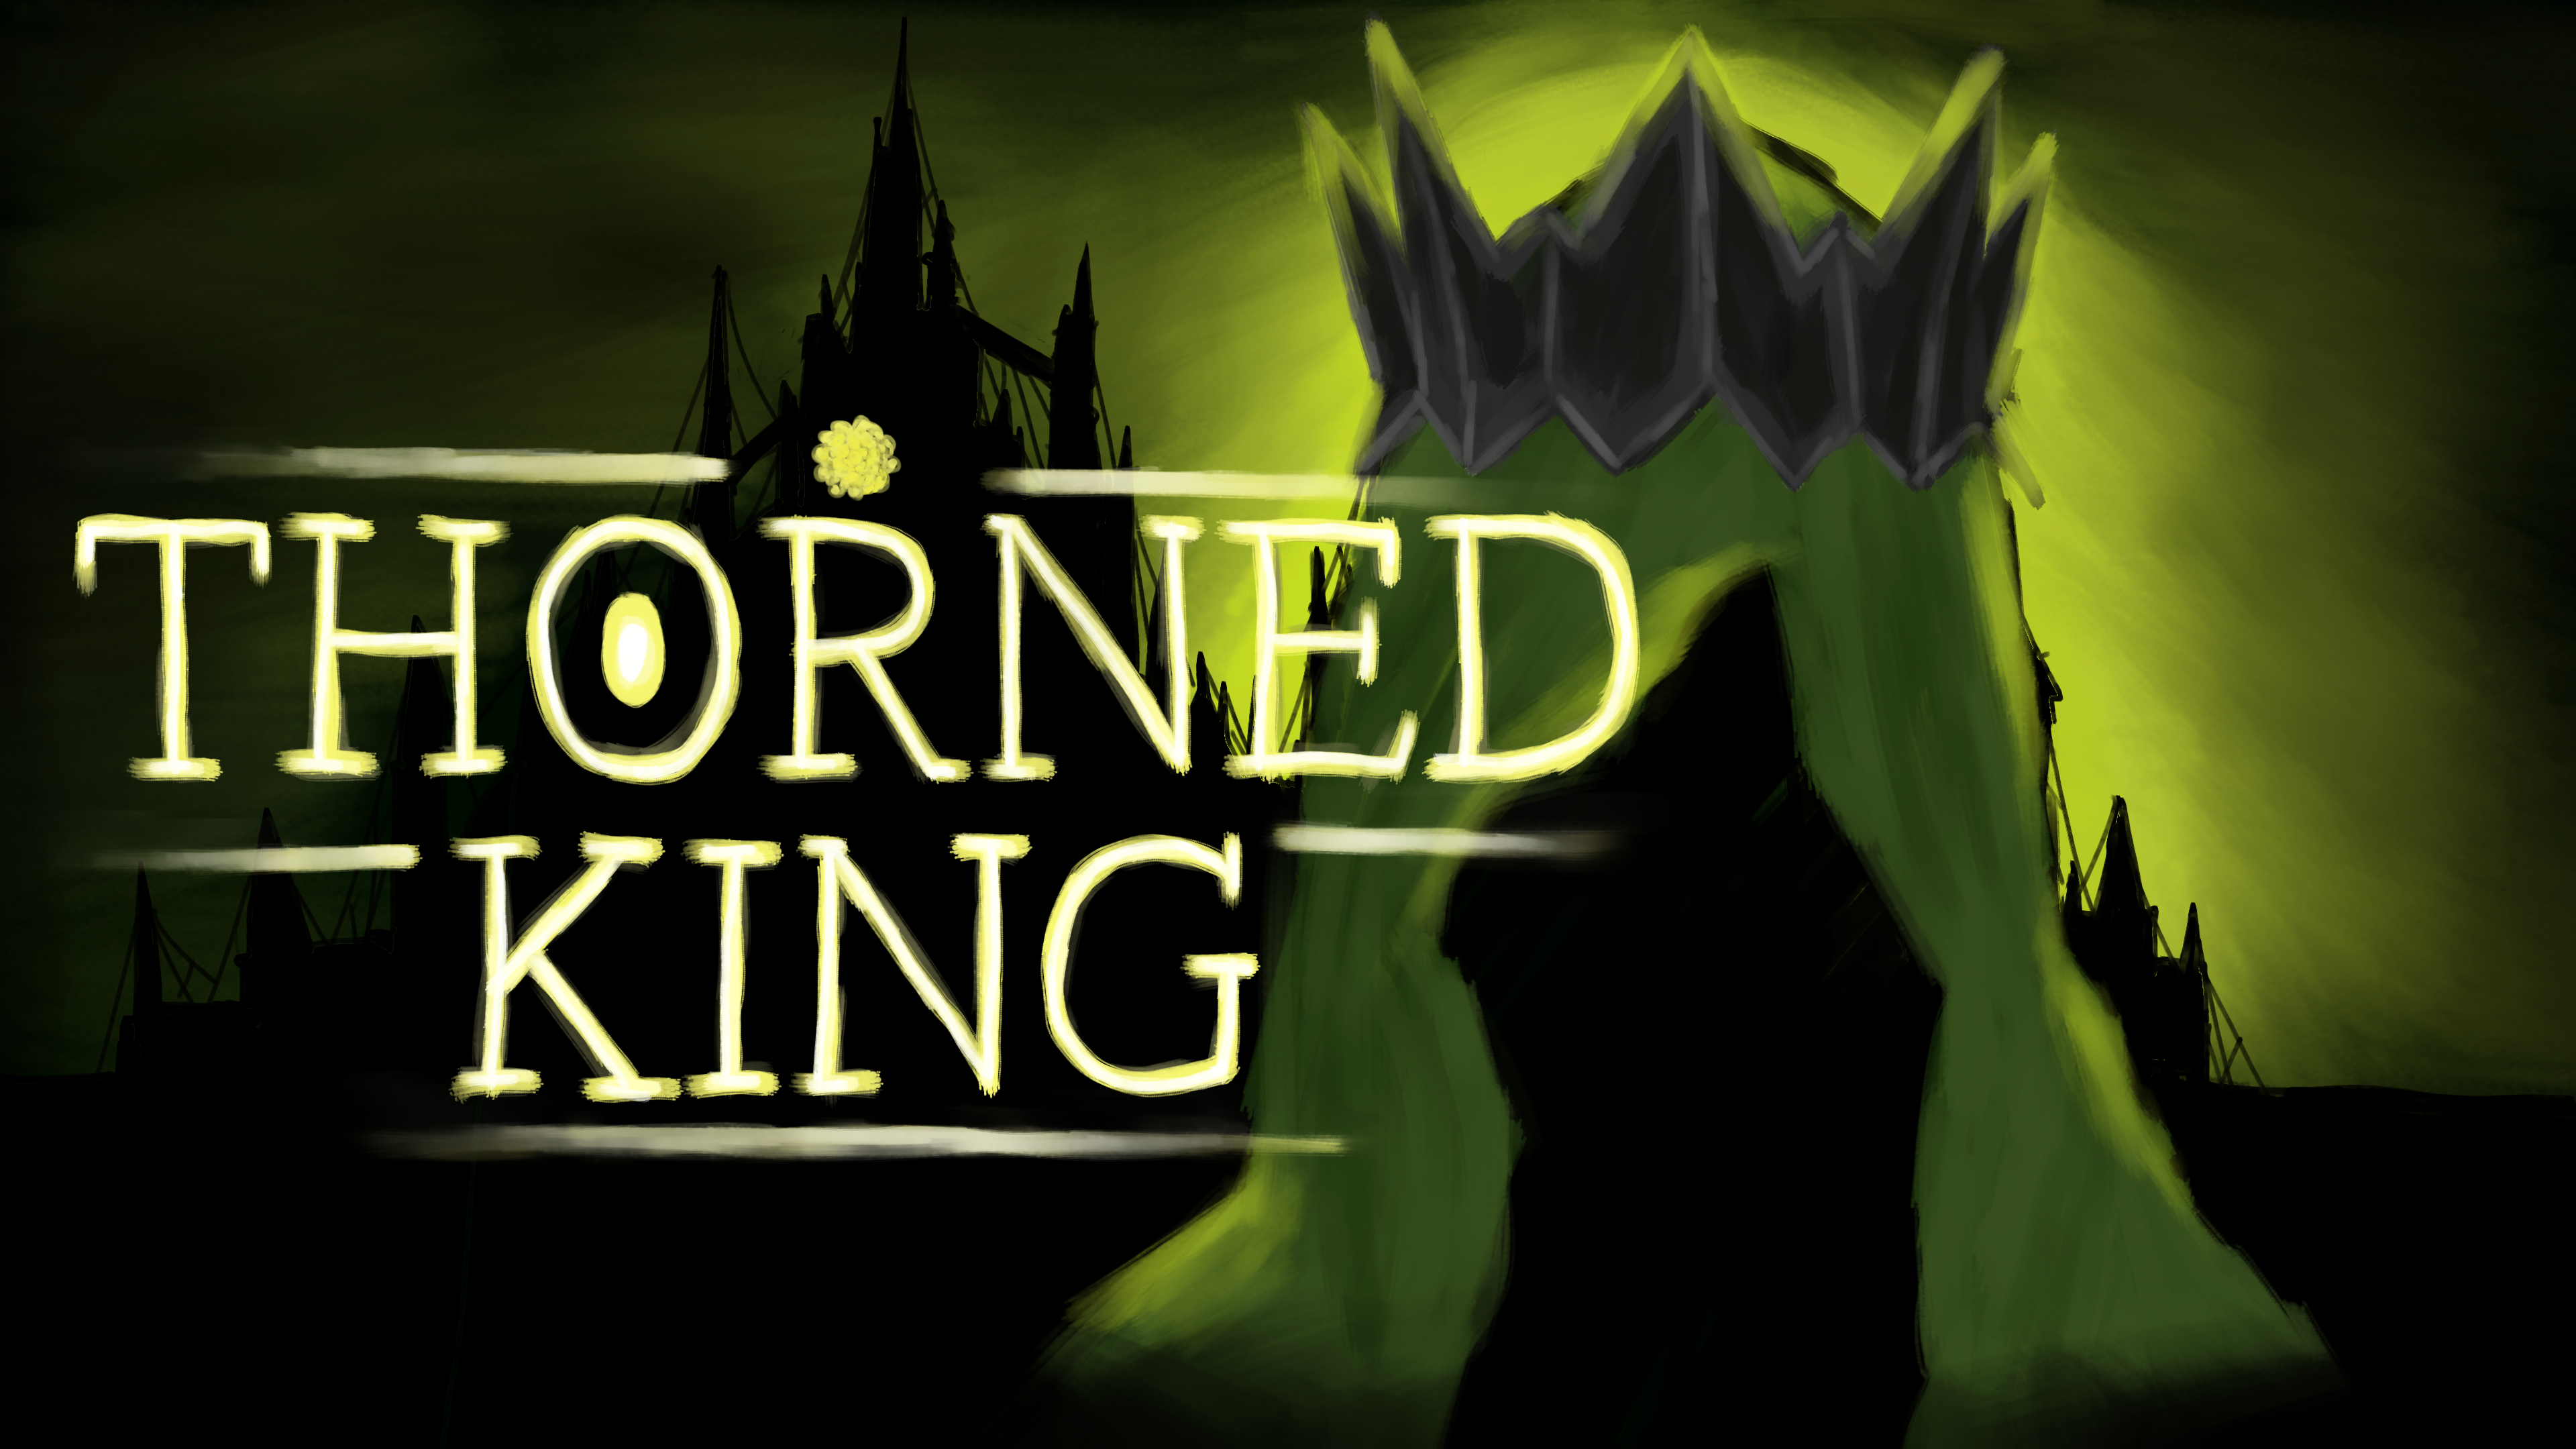
\includegraphics[width=1\textwidth]{images/Krita_ThornedKing.png}
	\label{fig:meinbild}
\end{figure}

\begin{center}
	 Version : 0.0.5 Prototyp
\end{center}


\end{titlepage}
\pagenumbering{arabic}
%------------------ Vorwort, Kurzfassung, Verzeichnisse ------------------------

%\kurzfassung
%Eine Kurzfassung

\tableofcontents										% Inhaltsverzeichnis
%\listoffigures
%\lstlistoflistings

% Du musst nicht alles beschreiben aber du kannst :) Neues Game yey
%------------------ Kapitel ----------------------------------------------------
\chapter{Spielidentität}
„Thorned King“ ist ein First-Person-Dungeon-Crawler, dessen Spielfortschritt auf dem Wissen des Spielers
über die Welt basiert. Dabei kämpft sich der Spieler als Abenteurer durch ein dornenüberwuchertes Schloss
und deckt so nach und nach dessen Geheimnisse auf.
\section{Unique Selling Points}
„Thorned King“ bietet eine Meta-Progression, welche auf dem Wissen des Spielers aufbaut, das er im Laufe
seines Spieldurchlaufs ansammelt. Dieses Wissen kann angewendet werden, um anderen
Handlungssträngen nachzugehen und die Navigation in der Welt zu beeinflussen. 
\\
Dadurch kann der Spieler bei einem weiteren Spieldurchlauf durch z. B. Türen schreiten, indem er sie nicht
ansieht, um seinen Spielfortschritt zu verändern und somit in Teile des Spiels vordringen, in die man
eventuell eher im späteren Spieldurchlauf gekommen wäre. Dies ist eingeplant und soll je nach
Charakterprogression und Nichtspieler-Charakter-Interaktion wiederum neue Erkenntnisse bringen. Dadurch
muss der Spieler, um alles über das Spiel zu erfahren, es mehrmals auf verschiedene Weisen durchspielen.
\\ \\
Das Spiel verfolgt eine konsistente immersive Designphilosophie. Dazu zählt die Architektur des Schlosses,
die einen besonderen Fokus auf die räumliche Orientierung legt und reduzierte Führung durch UI-Elemente.
\\ \\
Zusätzlich verändert der persönliche Charakterfortschritt, wie der Spieler mit der Welt interagieren kann und
welche Möglichkeiten ihm für die Navigation durch das Schloss zur Verfügung stehen. Attribute haben einen
direkten Einfluss auf die Interaktion mit der Spielwelt.
\chapter{Gameplay}
	\section{Ziele des Spieler}
	Verschlossene Türen und Hindernisse sowie starke Gegner sollen dem Spieler Ziele geben, wo man im Spiel
	weiterkommt und in welche Gebiete man erst später kommen kann. 
	\\Der Spieler soll im Hinterkopf
	mindestens immer einen Ort haben, an dem er noch nicht war und erst durch das Fortschreiten von
	Ausrüstung oder Überwinden von Hindernissen kommen kann. Somit kann man den Spieler durch das Spiel
	führen, ohne ihn direkt einzuschränken und an die Hand zu nehmen.
	\section{Spielmechaniken}
		\subsection{Charakter Erstellung und Anpassung}
		Der Spieler kann seinen Charakter anpassen. Dabei ändern die Attribute nicht nur Schaden oder Leben,
		sondern können auch entscheiden, wie der Spieler mit der Welt interagiert.
		\\ Die Vorgeschichte des
		Charakters kann einen passiven Effekt haben, wodurch eine indirekte Schwierigkeitsauswahl geschaffen
		wird.
		\\ Beispiel: Geschicklichkeit lässt einen höher springen oder Stärke lässt einen eine Kiste schieben, die
		man vorher nicht schieben konnte.
		\subsection{First-Person Kampfsystem}
		Angriffe können aufgeladen werden, um extra Schaden zu verursachen. Dies wird durch eine Anzeige
		verdeutlicht, wann der Schlag voll aufgeladen ist. Zusätzlich gibt es kritische Punkte, die auf den Gegnern
		verteilt sein können.
		\\ Beispiel: Ein aufgeladener Schlag auf den Kopf eines Gegners verursacht extra
		Schaden. Dazu kann man bis zu 2 Zauber während dem Kampf nutzen.
		
		\pagebreak
		\subsection{Interaktion mit der Welt}
		Der Spieler kann Gegenstände wie Tische und Bücher anheben, bewegen und werfen sowie mit Dingen
		interagieren, wie Hebel.
		\\ Damit eröffnet man mehr Möglichkeiten, Rätsel zu implementieren und alternative
		Wege zu finden, um durch das Schloss zu navigieren.
		\subsection{Nicht-Spieler-Charakter Interaktionen}
		Der Spieler kann durch Nicht-Spieler-Charaktere Quests erhalten, neue Gegenstände und Items, Tipps, wie
		man durch die Welt navigiert, sowie wird durch diese Handlung die Story der einzelnen Nicht-SpielerCharaktere fortgeführt.
		\\ Einige Nicht-Spieler-Charaktere bieten die Möglichkeit, Gegenstände zu kaufen.
		Andere wiederum können einem neue Fähigkeiten beibringen.
		\subsection{Ausrüstung/Item und Ressourcenmanagement}
		Items sowie neue Ausrüstung kann gefunden, gekauft oder durch Quests verdient werden.
		Dabei unterscheidet man zwischen Waffen, Ausrüstung um Attribute zu verbessern, Runen für das Wirken
		von Zaubern oder Konsumgütern die den Spieler beim Kampf oder der Exploration unterstützen. 
	\section{Steuerung}
	\begin{table}[]
		\centering
		\begin{tabular}{|l|l|l|}
			\hline
			Bewegung                & W/A/S/D          & Linker Stick             \\ \hline
			Springen                & Leertaste        & A                        \\ \hline
			Umschauen               & Maus Bewegung    & Rechter Stick            \\ \hline
			Angreifen               & Linke Maustaste  & Rechte Schultertaste     \\ \hline
			Blocken/Sekundärangriff & Rechte Maustaste & Linke Schultertaste      \\ \hline
			Zauber 1                & Q                & X                        \\ \hline
			Zauber 2                & R                & Y                        \\ \hline
			Drucken                 & STRG             & Rechter Stick eindrücken \\ \hline
			Interaktion             & E                & B                        \\ \hline
			Schnellzugriff Item 1   & 1                & D-Pad hoch               \\ \hline
			Schnellzugriff Item 2   & 2                & D-Pad rechts             \\ \hline
			Schnellzugriff Item 3   & 3                & D-Pad unten              \\ \hline
			Schnellzugriff Item 4   & 4                & D-Pad links              \\ \hline
		\end{tabular}
	\end{table}
	\pagebreak
	\section{Progression}
		\subsection{Charakter Progression}
		Der Spieler kann neue Ausrüstung finden, kaufen oder durch Quests verdienen, die er abhängig von seinen
		Attributen nutzen kann oder nicht.\\
		Durch das Besiegen von Gegnern, sowie das Erfüllen von Quests, erhält der Spieler Erfahrung. Wenn dieser
		genug angehäuft hat, erhält er ein Level Up. Dadurch kann er eins seiner Attribute an einem Speicherpunkt
		verbessern. 
		\subsection{Meta-Progression}
		Im Verlauf des Spiels enthüllen Spieler Geheimnisse und verborgene Regeln des Schlosses.
		Dieses Wissen ermöglicht es ihnen neue Wege zu finden, sowie Kämpfe und Situationen anders zu
		bewältigen. 
		So kann es beispielsweise relevant sein, ob der Spieler eine Tür vorwärts oder rückwärts durchschreitet, da
		diese abhängig davon in unterschiedliche Räume führt. 
		\\Andere Geheimnisse verändern die Navigation,
		enthüllen andere Handlungsstränge mit Nicht-Spieler-Charakteren oder ermöglichen einen früheren Zugang
		zu Bereichen des Schlosses, die man eigentlich erst später betritt.
		Mehrere Spieldurchläufe, sowie unterschiedliche Wege durch die Welt, enthüllen nach und nach mehr
		Geheimnisse des Schlosses und erweitern das Verständnis des Spielers über dessen Regeln und
		Zusammenhänge.
		 Dies geht so weit, dass man erst manche Teile des Schlosses nach mehrfachen
		Durchspielen betreten kann.
	\section{Speicherorte}
	Verteilt im Schloss findet der Spieler Speicherorte. Dort kann er seinen Spielfortschritt speichern, sowie die
	Attribute seines Charakters nach einem Levelaufstieg verbessern.
	\section{Verlieren}
	Wenn das Leben des Spielers auf 0 sinkt, hat er verloren und kann einen vorherigen Speicherstand laden.
	Wenn man stirbt, verliert man seine Progression bis zum letzten Speicherpunkt. 
\chapter{Systeme}
	\section{Kampfsystem}
	Der Spieler nutzt ein Fadenkreuz und seine ausgerüstete Waffe um Gegner anzugreifen. Dazu kann der
	Spieler seinen Angriff aufladen. Dies wird anhand des Fadenkreuzes angezeigt.
	\\ Je nach Waffe verändert sich
	die Eigenschaft und der Schaden der Waffe, wenn sie voll aufgeladen ist. Gegner können Schwachstellen
	haben und Blockstellen haben, die keinen Schaden zulassen.
	Die Angriffe des Spielers und der Gegner können verschiedene Schadensarten mit unterschiedlichen
	Eigenschaften besitzen. 
	\section{Ausrüstung}
	Waffen können Nah- oder Fernkampfwaffen sein und haben verschiedene Eigenschaften.
	Diese benötigen auch bestimmte Attribute um genutzt werden zu können.
	
		\begin{figure}[h]
		\centering
		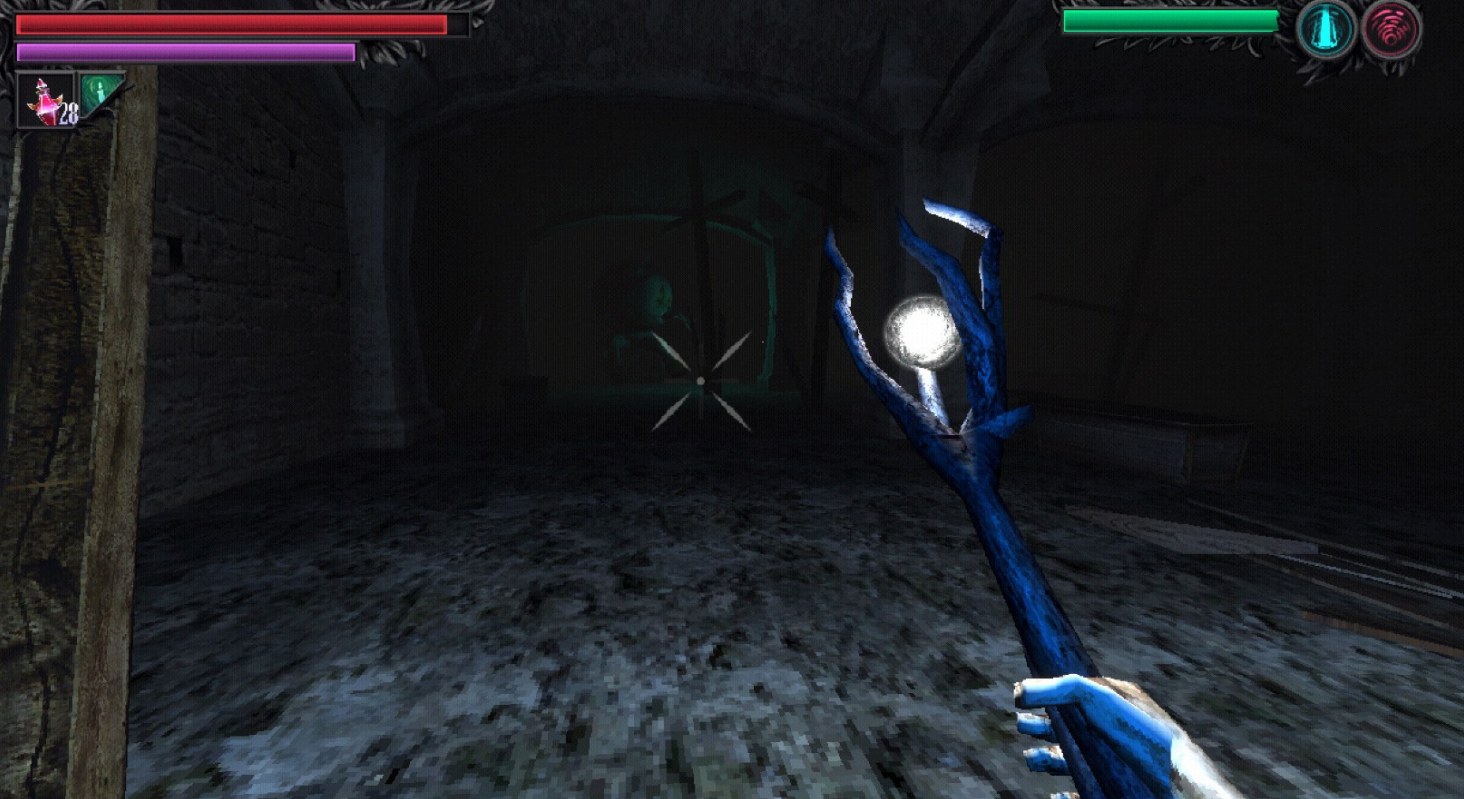
\includegraphics[width=0.7\textwidth]{images/LunacidKampf.png}
		\label{fig:meinbild}
	\end{figure}
	
		\begin{table}[]
		\centering
		\begin{tabular}{|l|l|l|}
			\hline
			Normaler Schaden                & Wird von Rüstung geblockt                     \\ \hline
			Feuer                & Kann Verbrennung auslösen                            \\ \hline
			Eis               & Kann verlangsamen               \\ \hline
			Licht               & Macht extra Schaden gegen Dunkelheit      \\ \hline
			Dunkelheit &Ignoriert Rüstung      \\ \hline
			Gift                &Verursacht Schaden über Zeit                                         \\ \hline
		\end{tabular}
	\end{table}
	Zauber kosten Mana und können während dem Kampf genutzt werden.
	\section{Ausrüstung}
	Waffen können Nah- oder Fernkampfwaffen sein und haben verschiedene Eigenschaften.
	Diese benötigen auch bestimmte Attribute um genutzt werden zu können.
			\begin{table}[]
		\centering
		\begin{tabular}{|l|l|l|}
			\hline
			Primäre Schadensart     & Verursachter Schaden \\ \hline
			Zusätzliche Schadensart (Optional)                 & Kann Verbrennung auslösen                            \\ \hline
			Reichweite               	& Kann verlangsamen               \\ \hline
			Angriffsgeschwindigkeit               & Macht extra Schaden gegen Dunkelheit      \\ \hline
			Kritischer Schaden &Ignoriert Rüstung      \\ \hline
			Blockkraft                &Verursacht Schaden über Zeit                                         \\ \hline
		\end{tabular}
	\end{table}
	
	Zusätzlich kann man Kleidung finden, die zusätzlichen Schutz und Verbesserungen bietet, entsprechend
	ihrer Eigenschaften. Dabei unterscheidet man zwischen Helmen und Kleidung.
	Helme können zusätzliche immersive Effekte haben, wie beispielsweise das Einschränken des Sichtfeldes
	
		\begin{table}[]
		\centering
		\begin{tabular}{|l|l|l|}
			\hline
			Schutz vor bestimmten Schadensarten      & Negiert eingehenden Schaden \\ \hline
		\end{tabular}
	\end{table}
	
	Ringe und Amulette verstärken Attribute oder geben besondere Boni.
	Runen verleihen einem die Möglichkeit Zauber zu wirken.
	\pagebreak
	\section{Attributsystem}
	Spieler erhalten durch einen Levelaufstieg einen Lernpunkt. Dieser kann bei Speicherorten genutzt werden,
	um ein Attribut zu erhöhen. Ab einer bestimmten Attributgrenze können Charaktere dann mit anderen
	Dingen interagieren oder schalten Fähigkeiten frei. 

	% Please add the following required packages to your document preamble:
	% \usepackage{graphicx}
\begin{table}[ht]
	\centering
	\begin{tabular}{|l|p{9cm}|}
		\hline
		Stärke & Erhöht den Schaden von Waffen. Man kann abhängig von der Stärke verschieden schwere Gegenstände heben und bewegen. \\ \hline
		
		Geschicklichkeit & Erhöht Angriffsgeschwindigkeit und Sprunghöhe. \\ \hline
		
		Intelligenz & Erhöht Mana und ermöglicht das Verstehen verschiedener Schriften. \\ \hline
		
		Glück & Erhöht die Chance, Schaden zu entgehen, wertvolle Beute zu finden und kritische Treffer zu landen. \\ \hline
		
		Konstitution & Erhöht das Leben. \\ \hline
		
		Geschwindigkeit & Erhöht die Laufgeschwindigkeit. \\ \hline
	\end{tabular}
\end{table}

Lernpunkte können bei Nicht-Spieler-Charakteren für besondere Fähigkeiten eingetauscht werden.
\chapter{Geschichte und Setting}
„Thorned King“ spielt in einem düsteren Mittelalter Fantasy Setting, indem tapfere Helden gegen die Mächte
des Bösen kämpfen.
Dein Leben wird auf den Kopf gestellt, nachdem gewaltige Ranken in deiner Heimat auftauchen. Sie
verschlingen alles, was sich ihnen in den Weg stellt, reißen Häuser nieder und hinterlassen nur Tod und
Verwüstung. Dabei verlierst du nicht nur dein Zuhause, sondern auch deine Familie.
Ohne etwas zu verlieren, schließt du dich einer Gruppe Abenteurern an, die entschlossen sind die Ursache
zu finden und zu vernichten. Doch die Wochenlange Reise fordert ihren Tribut und du kommst allein und
erschöpft am Epizentrum an.\\
Ein von Dornenranken überwuchertes Schloss. Von Rache getrieben machst du dich auf den Weg die Quelle
des Fluchs zu vernichten. 
\chapter{Artstyle}
Der Artstyle soll Lowpoly und Pixelated sein damit die Erstellung vereinfacht und beschleunigen wird. Dabei
orientiert man sich an alten PS1 Spielen, ähnlich wie Kingsfield. \\
Man kombiniert eine Grundpalette und eine Variation von Assets um eine Variation an Gebieten zu bieten
ohne zu viele Assets produzieren zu müssen.
Es sollen nicht nur düstere Monumente gezeigt werden, wie es typisch ist bei solchen Spielen, sondern auch
die Außenwelt. 
\begin{figure}
\centering
\begin{minipage}{.5\textwidth}
	\centering
	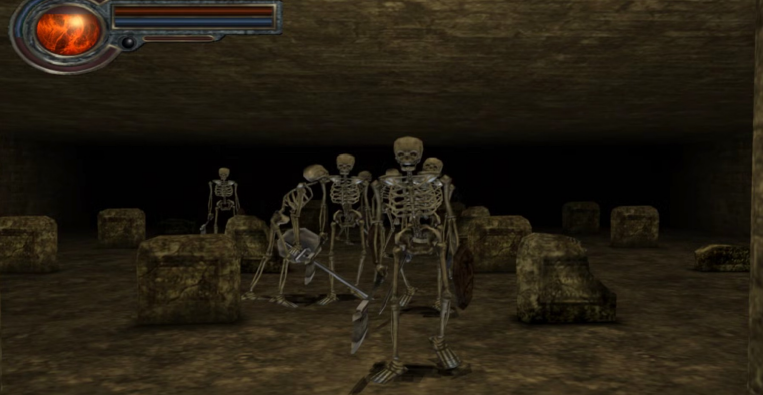
\includegraphics[width=.8\linewidth]{images/Kingsfield_Artstle.png}
	\captionof{figure}{Kingsfield}
	\label{fig:test1}
\end{minipage}%
\begin{minipage}{.5\textwidth}
	\centering
	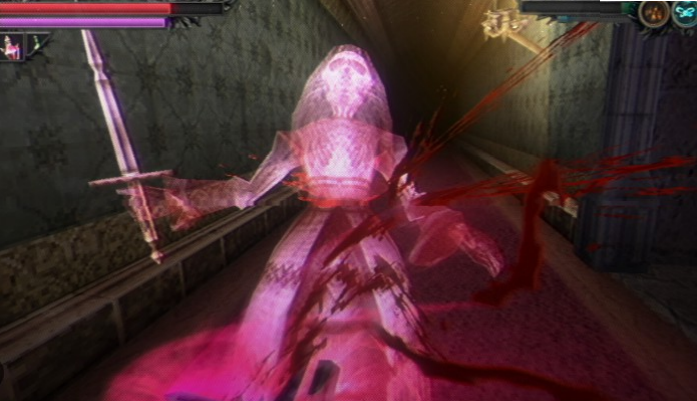
\includegraphics[width=0.8\linewidth]{images/Lunacid_Artstyle.png}
	\captionof{figure}{Lunacid}
	\label{fig:test2}
\end{minipage}
\end{figure}

\pagebreak
Um sich von anderen Dungeon-Crawlern abzuheben, setzt „Thorned King“ bewusst auf verschiedene
Farbpaletten. Dabei sollen die hellen, offenen Oberflächen des Schlosses ein Kontrast zu den dunklen und
bedrückenden Bereich im Inneren des Schlosses darstellen. 
\\
\begin{figure}
\centering
\captionsetup{font=small}
\begin{minipage}{.5\textwidth}
	\centering
	\captionsetup{font=small}
	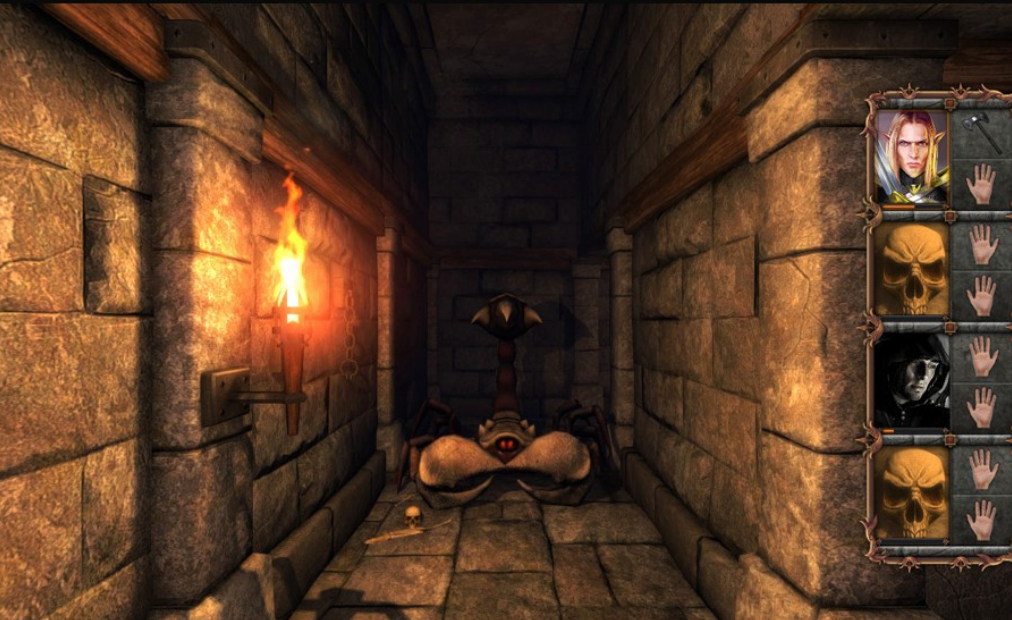
\includegraphics[width=.8\linewidth]{images/Dunkle_Farbpalette.png}
	\captionof{figure}{Beispiel dunkle Farbpalette }
	\label{fig:test1}
\end{minipage}%
\begin{minipage}{.5\textwidth}
	\centering
	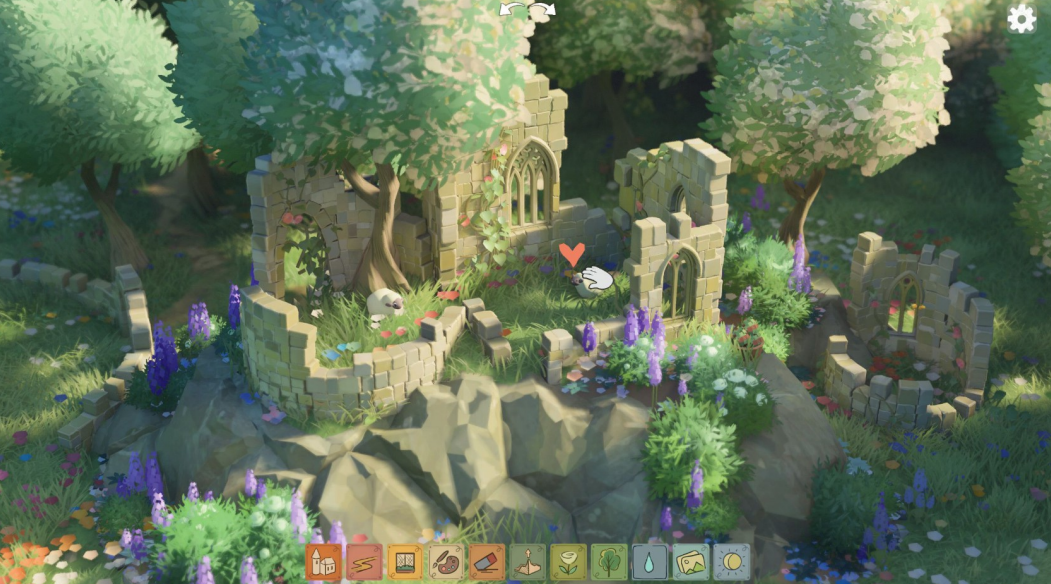
\includegraphics[width=0.8\linewidth]{images/helleFarbpalette.png}
	\captionof{figure}{Beispiel helle Farbpalette}
	\label{fig:test2}
\end{minipage}
\end{figure}
\\
Darüber hinaus werden, bei dem Erstellen der Assets für die Burgen und Gänge, die Burgen und Schlösser
und deren Architektur aus dem Saarland als Vorbild genommen. 
\begin{figure}
\centering
\captionsetup{font=small}
\begin{minipage}{.5\textwidth}
	\centering
	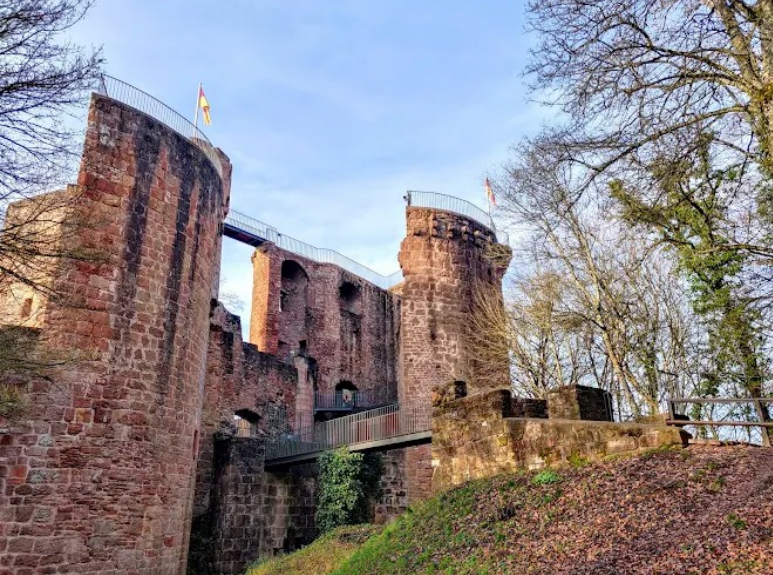
\includegraphics[width=.8\linewidth]{images/Burg Montclair (Mettlach).png}
	\captionof{figure}{Burg Montclair (Mettlach) }
	\label{fig:test1}
\end{minipage}%
\begin{minipage}{.5\textwidth}
	\centering
	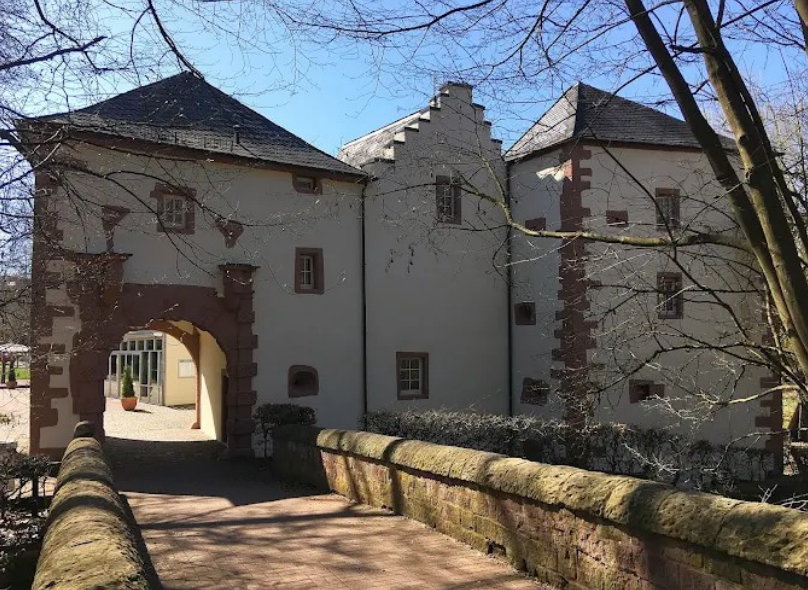
\includegraphics[width=0.8\linewidth]{images/Burg Kerpen (Illingen).png}
	\captionof{figure}{Burg Kerpen (Illingen)}
	\label{fig:test2}
\end{minipage}
\end{figure}

\chapter{Sound}
	\section{Soundeffekte}
	Soundeffekte unterstützen alle Interaktionen, um möglichst viel Immersion beim Spieler zu erzeugen. Dabei
	wird ein eigen geschriebenes Soundsystem verwendet. Dieses kommt in allen Bereichen des Spiels zum
	Einsatz. Von der Nutzung der UI bis hin zum Kampf.
	\section{Ambient-Sound}
	Der Ambient-Sound soll die Stimmung der Szene unterstreichen.\\
	\\
	\href{https://www.youtube.com/watch?v=_IWZyPWsSvQ}{Im inneren des Schlosses (Link)}
	\\
	\href{https://www.youtube.com/watch?v=xNN7iTA57jM}{An der Oberfläche des Schlosses (Link)}
	
%	Im inneren des Schlosses : [ https://www.youtube.com/watch?v=_IWZyPWsSvQ ]
%	An der Oberfläche des Schlosses : [ https://www.youtube.com/watch?v=xNN7iTA57jM ]
	\section{Musik}
	Die Musik bewegt sich zwischen düster und hoffnungsvoll. So ändert sich die Stimmung, sobald man einen
	anderen Abenteurer findet oder sich ins Innere des Schlosses vorwagt. An ausgewählten Stellen wird
	bewusst vollständig auf Musik verzichtet um Spannung und Atmosphäre zu erzeugen.
	\\
	\href{ https://youtu.be/pn6-2hrTfjk?si=z8jH8ErvW_UlgCwL&t=1223}{Beispiel : Simon Heath Dungeon SynthLink}
	
\chapter{Technische Umsetzung}
Für die technische Umsetzung wird die Unity-Engine genutzt, sowie Tools aus dem Unity-Asset-Store um
die Entwicklung zu beschleunigen.

\begin{table}[ht]
	\centering
	\begin{tabular}{|l|p{9cm}|}
		\hline
		Dialogs und Quests & Pixelcrusher Dialogsystem \\ \hline
		
		Schnellere Entwicklung & Reload System \\ \hline
		
	Schnellere Entwicklung  & Prefab Brush
	 \\ \hline
		
		Occlusion Culling  &Perfect Culling \\ \hline
		
	Pathfinding & A* Pathfinding Project Pro \\ \hline
		
	AI  & Behavior Designer Pro 3 \\ \hline
		Art   &Art Assets die angepasst werden. Dabei werden
		nur uninteressante Objekte wie Steine und Co
		ersetzt. \\ \hline
	\end{tabular}
\end{table}


\chapter{Roadmap}
	\section{Scope}
	Der Spieler soll für den ersten Spieldurchlauf knapp 10 Stunden benötigen, aber dafür soll der
	Wiederspielwert im Vordergrund stehen. 
	\\Der Prototyp beinhaltet ein Level von 30 Minuten.
	\section{Prototyp Milestones}
	Milestone 1. Kampf und Bewegungsmechanik sind implementiert \\
	Milestone 2. Abschluss aller wichtigen Mechaniken \\
	Milestone 3. Prototyp Level abgeschlossen  \\
\chapter{Marketing}
	\section{Zielgruppe}
	Das Spiel „Thorned King“ richtet sich an die Fans klassischer Rollenspiele und Dungeon Crawler der frühen
	2000er Jahre. Die Zielgruppe sind daher eher ältere Spieler, schätzungsweise zwischen 30 und 50 Jahren
	sowie Fans atmosphärischer First-Person Rollenspiele mit Nostalgischen Charme und einen Fokus auf
	Erkundung und Immersion. 
	\section{Social Media}
	Die deutsche Rollenspielcommunity erfährt durch das Gothic Remake einen neuen Aufschwung.
	Dadurch sind gerade Content Creator offen für neue Rollenspiele aus dem deutschsprachigen Raum.
	\\
	Dies bietet die Möglichkeit die Community frühzeitig in die Entwicklung von „Thorned King“ einzubeziehen
	durch Entwickler-Updates, Einblicke in den Entwicklungsprozess, sowie Playtests und Feedbackrunden. 
	\section{Plattform und Monetarisierung}
	Das Spiel wird zunächst ausschließlich auf Steam erscheinen, mit Windows, Linux und Steamdeck Support.
	\section{Lokalisation}
	Das Spiel wird Anfangs in Deutsch und Englisch verfügbar sein
	\section{Erweiterungen}
		Spiele leben heutzutage durch Updates und Erweiterungen nach dem Release. Das Spiel soll auch nach
		Release mindestens noch 6 Monate Support erhalten. 
	\section{Ähnliche Spiele und deren Umsatz}
\begin{figure}
	\centering
	\captionsetup{font=small}
	\begin{minipage}{.5\textwidth}
		\centering
		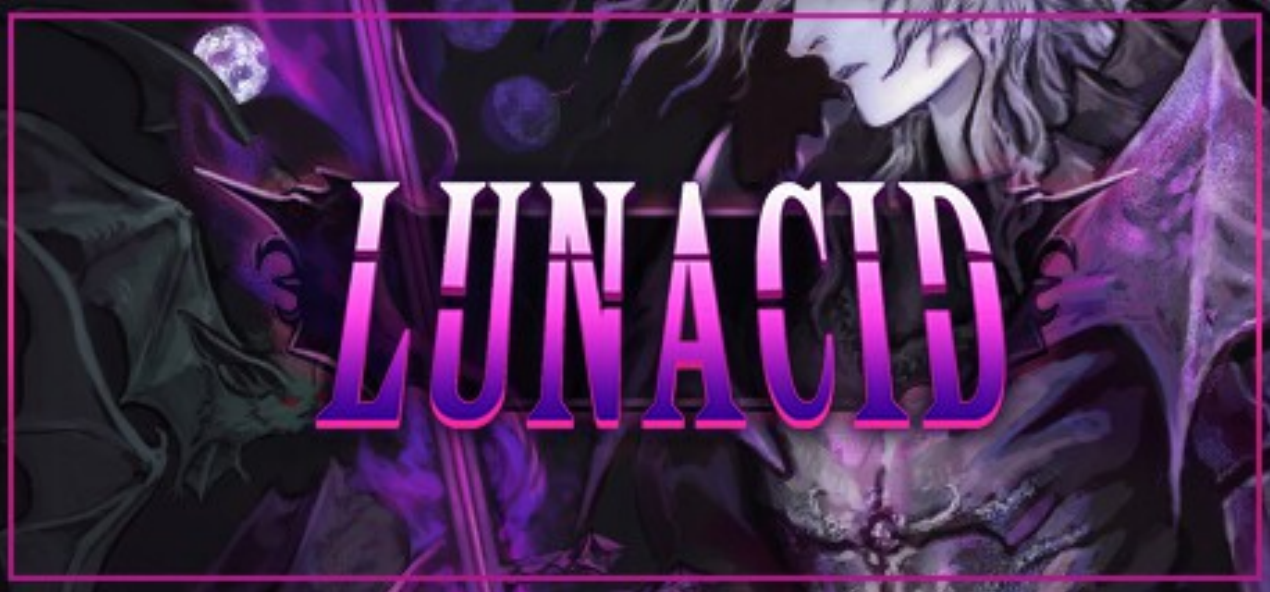
\includegraphics[width=.7\linewidth]{images/Lunacid_Steam_Bild.png}
		\label{fig:test1}
	\end{minipage}%
	\begin{minipage}{.5\textwidth}
		\centering
		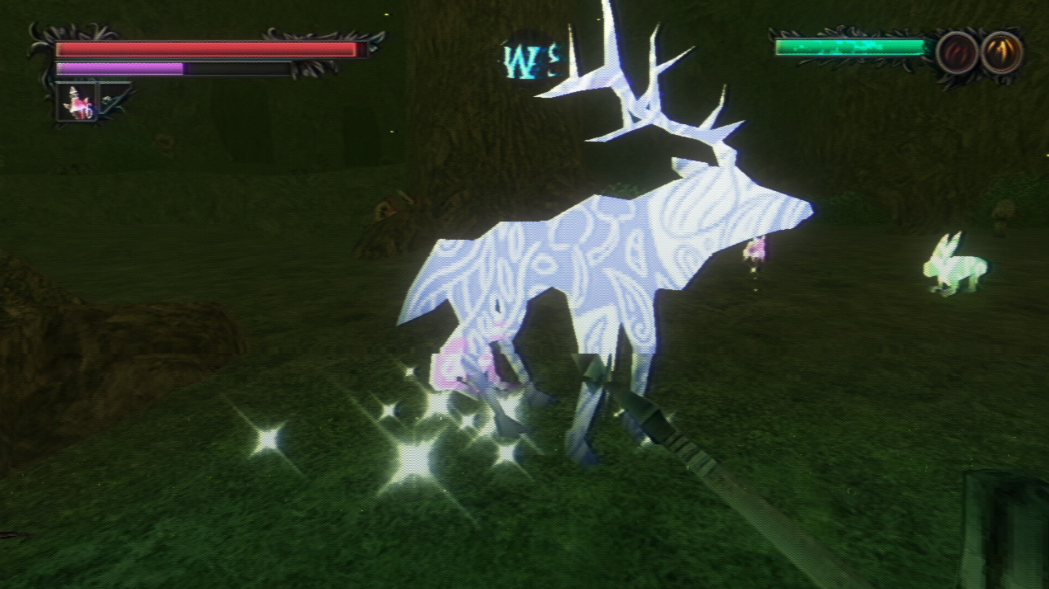
\includegraphics[width=0.7\linewidth]{images/Lunacid_Steam_Bild_2.png}
		\label{fig:test2}
	\end{minipage}
\end{figure}

Preis 13.79€ \\
~3.100.000 € Umsatz \\
~328.000 Verkäufe \\
Anzahl der Entwickler : 1 \\

\begin{figure}
	\centering
	\captionsetup{font=small}
	\begin{minipage}{.5\textwidth}
		\centering
		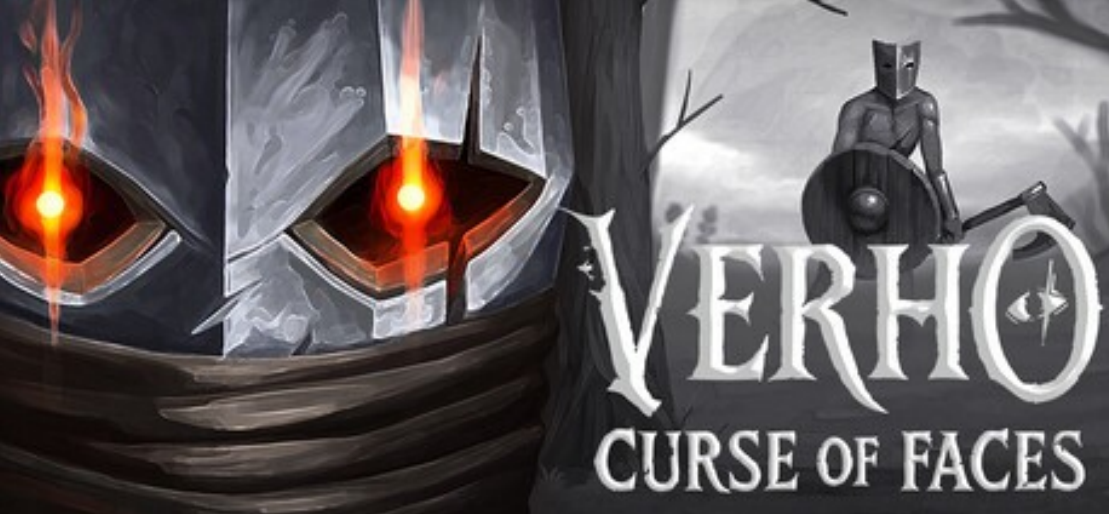
\includegraphics[width=.7\linewidth]{images/Verho_Steambild_1.png}
		\label{fig:test1}
	\end{minipage}%
	\begin{minipage}{.5\textwidth}
		\centering
		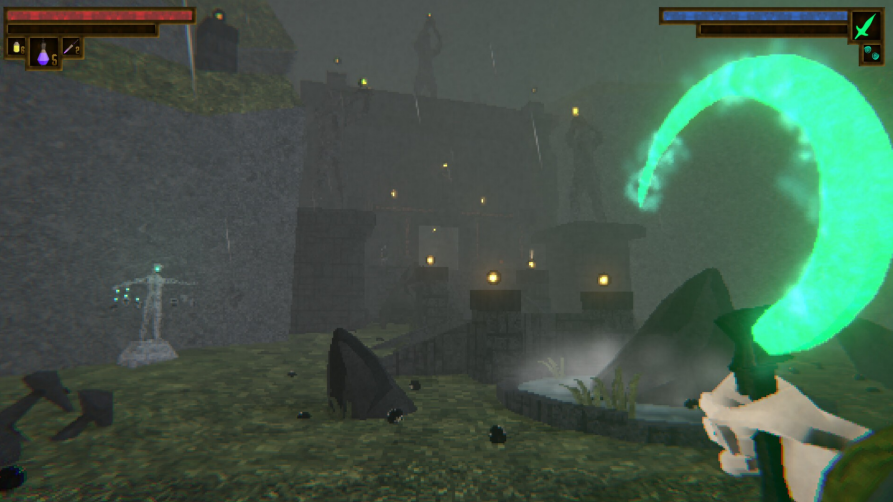
\includegraphics[width=0.7\linewidth]{images/Verho_Steambild_2.png}
		\label{fig:test2}
	\end{minipage}
\end{figure}
Preis : 19.99 € \\	
~370.000 € Umsatz \\
~ 23.000 Verkäufe \\
Anzahl der Entwickler : 7 \\

\begin{figure}
	\centering
	\captionsetup{font=small}
	\begin{minipage}{.5\textwidth}
		\centering
		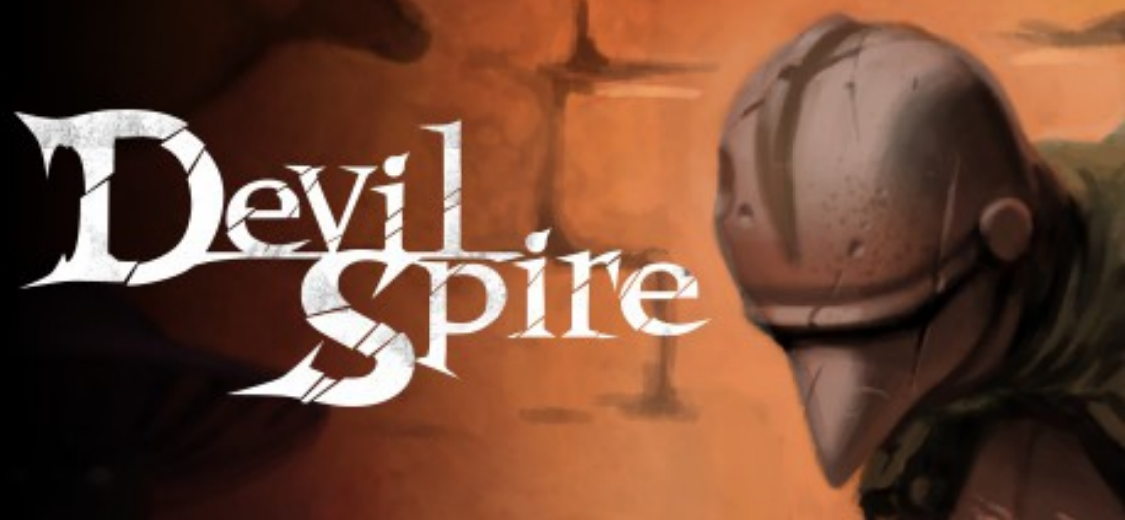
\includegraphics[width=.7\linewidth]{images/DevilSpire_SteamBild_1.png}
		\label{fig:test1}
	\end{minipage}%
	\begin{minipage}{.5\textwidth}
		\centering
		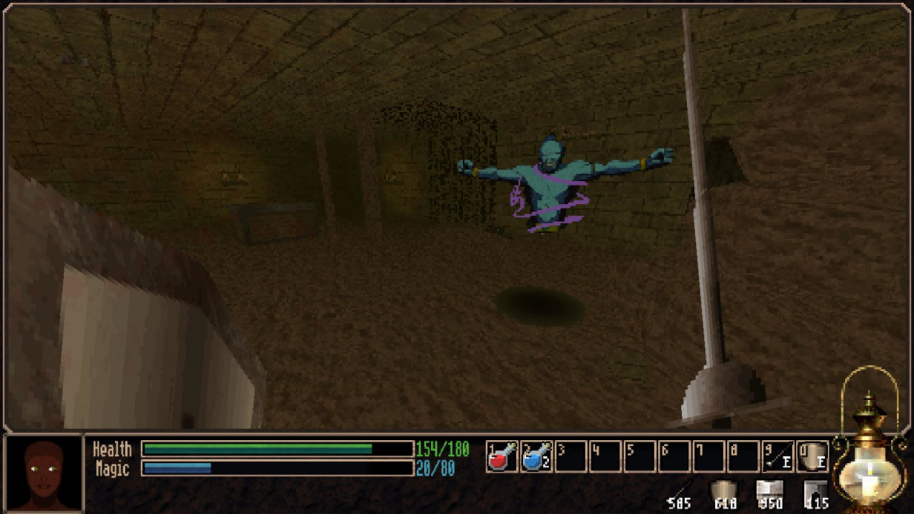
\includegraphics[width=0.7\linewidth]{images/DevilSpire_SteamBild_2.png}
		\label{fig:test2}
	\end{minipage}
\end{figure}

Preis : 9.99€ \\
~84.000 € Umsatz \\
~ 16.600 Verkäufe \\
Anzahl der Entwickler : 3\\

Alle Angaben wurden durch 	\href{gamalytic.com}{gamalytic.com} getroffen und können in Zukunft abweichen (2026)

%------------------ Anhänge ----------------------------------------------------
\begin{appendix}
	%\chapter{Selbstständigkeitserklärung}

\begin{description}

\item[$\Box$] Diese Arbeit habe ich selbstständig verfasst und keine anderen als die angegebenen Quellen und Hilfsmittel verwendet.\\

\item[$\Box$] Diese Arbeit wurde als Gruppenarbeit angefertigt. Meinen Anteil habe ich selbstständig verfasst und keine anderen als die angegebenen Quellen und Hilfsmittel verwendet.\\

Namen der Mitverfasser:
\vspace{3cm}

Meine eigene Leistung ist:
\vspace{3cm}

\end{description}

\vspace{3cm}

\begin{minipage}[t]{3cm}
	\rule{3cm}{0.5pt}
	Datum
\end{minipage}
\hfill
\begin{minipage}[t]{9cm}
	\rule{9cm}{0.5pt}
	Unterschrift der Kandidatin/des Kandidaten
\end{minipage}
	% Selbstständigkeitserklärung
\end{appendix}


\end{document}
